%%%%%%%%%%%%%%%%%%%%%%%%%%%%%%%%%%%%%%%%%
% baposter Landscape Poster
% LaTeX Template
% Version 1.0 (11/06/13)
%
% baposter Class Created by:
% Brian Amberg (baposter@brian-amberg.de)
%
% License:
% CC BY-NC-SA 3.0 (http://creativecommons.org/licenses/by-nc-sa/3.0/)
%
%%%%%%%%%%%%%%%%%%%%%%%%%%%%%%%%%%%%%%%%%

%----------------------------------------------------------------------------------------
% PACKAGES AND OTHER DOCUMENT CONFIGURATIONS
%----------------------------------------------------------------------------------------

\documentclass[landscape,a0paper,fontscale=0.285]{baposter} % Adjust font scale/size

\usepackage{graphicx} % Required for including images
\graphicspath{{figs/}} % Directory in which figures are stored

\usepackage{amsmath} % For typesetting math
\usepackage{amssymb} % Adds new symbols to be used in math mode
\usepackage{mathtools}

\usepackage[numbers]{natbib}

\usepackage{booktabs} % Top and bottom rules for tables
\usepackage{enumitem} % Used to reduce itemize/enumerate spacing
\usepackage{palatino} % Use the Palatino font
\usepackage[font=small,labelfont=bf]{caption} % Required for specifying captions to tables and figures

\usepackage{multicol} % Required for multiple columns
\setlength{\columnsep}{1.5em} % Slightly increase the space between columns
\setlength{\columnseprule}{0mm} % No horizontal rule between columns

\newcommand{\compresslist}{ % Define a command to reduce spacing within itemize enumerate environments, this is used right after \begin{itemize} or \begin{enumerate}
\setlength{\itemsep}{1pt}
\setlength{\parskip}{0pt}
\setlength{\parsep}{0pt}
}

\definecolor{lightblue}{rgb}{0.145,0.6666,1} % Defines color of content box headers

\begin{document}

\begin{poster} {
headerborder=closed, % Adds a border around the header of content boxes
colspacing=1em, % Column spacing
bgColorOne=white, % Background color for the gradient on the left side of the poster
bgColorTwo=white, % Background color for the gradient on the right side of the poster
borderColor=lightblue, % Border color
headerColorOne=black, % Background color for the header in the content boxes (left side)
headerColorTwo=lightblue, % Background color for the header in the content boxes (right side)
headerFontColor=white, % Text color for the header text in the content boxes
boxColorOne=white, % Background color of the content boxes
textborder=roundedleft, % Format of the border around content boxes, can be: none, bars, coils, triangles, rectangle, rounded, roundedsmall, roundedright or faded
eyecatcher=true, % Set to false for ignoring the left logo in the title and move the title left
headerheight=0.1\textheight, % Height of the header
headershape=roundedright, % Specify the rounded corner in the content box headers, can be: rectangle, small-rounded, roundedright, roundedleft or rounded
headerfont=\Large\bf\textsc, % Large, bold and sans serif font in the headers of content boxes
%textfont={\setlength{\parindent}{1.5em}}, % Uncomment for paragraph indentation
linewidth=2pt % Width of the border lines around content boxes
}
%----------------------------------------------------------------------------------------
% TITLE SECTION
%----------------------------------------------------------------------------------------
%
{
\includegraphics[height=6.5em]{logo_cal.jpg}} % First university/lab logo on the left
{\bf\textit{\LARGE Robust Nonparametric Inference for Stochastic Interventions
    Under Multi-Stage Sampling}\vspace{0.01em}} % Poster title
{\textbf{Nima S.~Hejazi, Mark J.~van der Laan, and David C.~Benkeser} \\
  \textit{Group in Biostatistics \& Department of Statistics, University of
    California, Berkeley} \\
  \textit{Department of Biostatistics and Computational Biology, Emory
    University}} % Author names and institution
{
\includegraphics[height=6.5em]{logo_sph.jpg}} % Second university/lab logo on the right

%-------------------------------------------------------------------------------
% OVERVIEW
%-------------------------------------------------------------------------------

\headerbox{Overview \& Motivations}{name=overview,column=0,row=0}{

\begin{enumerate}\compresslist
\setlength\itemsep{0.5em}
\item We consider the problem of efficiently estimating the effect of a
 stochastic shift interventions for problem settings in which multi-stage
 sampling complicates the observed data structure.
\item We present a novel approach: an augmented targeted maximum likelihood
 estimator of a parameter defined as the outcome under a stochastic
 intervention with
  \begin{itemize}
    \item consistency and efficiency guarantees even under multi-stage
      sampling, and
    \item a form of multiple double robustness inherited from its constituent
      parts.
  \end{itemize}
\item The proposed nonparametric estimation procedure provably attains fast
  convergence rates even when incorporating machine learning estimators.
\item A recent software implementation --- the ``txshift'' R package --- has
  been developed for applying this methodology very generally, including for
  causal inference and variable importance analyses.
\end{enumerate}

%\vspace{0.3em} % When there are two boxes, some whitespace may need to be added
               % if the one on the right has more content
}

%-------------------------------------------------------------------------------
% INTRODUCTION
%-------------------------------------------------------------------------------

\headerbox{Introduction \& Data}
{name=introduction,column=1,row=0,bottomaligned=overview}{

\begin{itemize}\compresslist
\setlength\itemsep{0.5em}
\item We illustrate the utility of our approach by applying the new method and
  software in an investigation of the effects of immune response biomarkers on
  HIV vaccine efficacy.
\item \textit{Question of interest:} \textbf{How does risk of HIV infection
   differ under posited shifts of the distribution of an immune response in the
   vaccine arm of an efficacy trial?}
\item We simulate a data structure similar to that in the HVTN 505 HIV-1
  efficacy trial:
  \begin{itemize}
    \itemsep0.5pt
    \item About 2500 participants, with all observed cases matched to controls.
    \item Background $(W)$: sex, age, BMI, etc.
    \item Intervention $(A)$: immunomarkers (i.e., T-Cell profiles from ICS
      assay on HIV-1-stimulated PBMCs).
    \item Outcome $(Y)$: HIV-1 infection risk.
  \end{itemize}
\item \textit{Takeaway:} \textbf{Variable importance measure for ranking
   multiple immune responses by their utility as immunogenicity study endpoints
   in future HIV-1 vaccine trials.}
\end{itemize}
}

%-------------------------------------------------------------------------------
% Methodology cont.
%-------------------------------------------------------------------------------

\headerbox{Methodology II}{name=results,column=2,span=2,row=0}{


\vspace{-0.35em}
\begin{itemize}
\item The second approach is non-parametric and uses Kaplan-Meier's estimator
  defined as
\end{itemize}
\begin{equation*}
\widehat{S}(t) = \prod_{i : t(i) < t} \left(1 - \frac{d_i}{n_i}\right), \quad
t\geq 0,
\end{equation*}
where $d_i$ and $n_i$ are the respective numbers of death and individual at
risks at the ordered time $t^{(i)}, \ i = 1, \ldots, n$.
\begin{itemize}
\item Youlden et al. \cite{youlden2016ten} only uses patients for whom no
  occurrence of a second melanoma is observed, in the estimation of $S_1$ and
  ignores the other patients, which causes a bias.
\item Jewell corrects their estimator by including all the patients in the
  study.
\item The ones that were excluded by Youlden et al. \cite{youlden2016ten} still
  contain information about $\lambda_1$: those are censored observations at time
  $U$.
\end{itemize}
}

%-------------------------------------------------------------------------------
% REFERENCES
%-------------------------------------------------------------------------------

\headerbox{Principal References}{name=references,column=2,above=bottom}{
\renewcommand{\section}[2]{\vskip 0.05em} % remove "References" section title
\nocite{*} % Insert publications even if they are not cited in the poster
\tiny{ % Reduce the font size in this block
\setlength{\bibsep}{1pt}
\bibliographystyle{unsrt}
\bibliography{2018_acic}\compresslist
}
}

%-------------------------------------------------------------------------------
% CONTACT
%-------------------------------------------------------------------------------

\headerbox{Contact Information}{name=ack,column=3,aligned=references,above=bottom}{
% This block is as tall as the references block
  \textbf{N.S.~Hejazi}: \textsc{nhejazi@berkeley.edu} \\
  \textbf{M.J.~van der Laan}: \textsc{laan@berkeley.edu} \\
  \textbf{D.~C.~Benkeser}: \textsc{benkeser@emory.edu}
}

%-------------------------------------------------------------------------------
% CONCLUSION
%-------------------------------------------------------------------------------

\headerbox{Results \& Discussion}
{name=conclusion,column=2,span=2,row=0,below=results,above=references}{

\vspace{1em}
\begin{multicols}{2}

\begin{center}
\vspace*{-0.45cm}
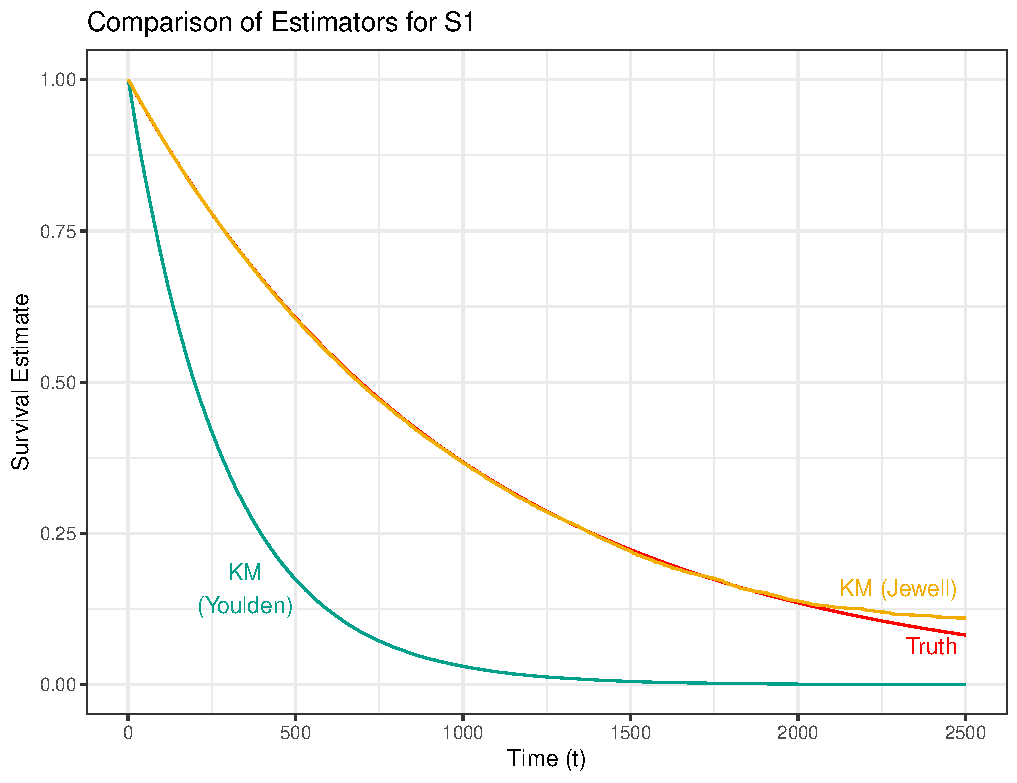
\includegraphics[scale=0.5]{s1_estim_compare}
\vspace{-1.5em}
\captionof{figure}{Average performance of estimators for $S_1$ for a sample of
 size $n = 1000$, over about $300$ simulations.}
\end{center}

\vspace{3em}

\begin{itemize}
  \setlength\itemsep{0.2em}
  \item The Kaplan-Meier estimator proposed by Youlden displays obvious bias.
  \item The estimates of the survival curve produced by Cox regression and the
    Kaplan-Meier estimator with the Jewell correction show no such bias.
  \item Under the Cox model, Cox regression will outperform other estimators ---
    it draws upon information across both subject groups over all time points.
  \item The Kaplan-Meier estimator exhibits a slight divergence from the truth
    in the right tail due to a well-studied finite-sample bias caused by
    censored observations.
  \item We display results for $n = 1000$ since this sample size is closest to
    that from the observational medical study we analyze.
\end{itemize}

\end{multicols}

}

%-------------------------------------------------------------------------------
% METHODS
%-------------------------------------------------------------------------------

\headerbox{Methodology I}{name=method,column=0,span=2,below=overview,bottomaligned=references}{
% This block's bottom aligns with the bottom of the conclusion block

\begin{itemize}
  \item Consider $O = (W, A, Y) \sim P_0 \in \mathcal{M}$, where no assumptions
    are placed on the statistical model containing $\mathcal{M}$ containing
    $P_0$.
  \item Rather than a deterministic intervention, consider a shift of the
    treatment (i.e., instead of $A = a$, consider $A = a + \delta$).
  \item To compare with the general linear model, the shift $\delta$ may be
    thought of as analogous to shifts in the slope of the regression line.
  \item To protect against positivity violations, make the shifting mechanism a
    function of the observed data: $d(a, w) = a + \delta$, if
    $a + \delta < u(w)$ and $d(a, w) = a$ otherwise.
\end{itemize}

Let's consider a simple statistical target parameter:
\begin{equation}
\Psi(P) = \mathbb{E}_P{\bar{Q}(d(A, W), W)},
\end{equation}
for which the efficient influence function (EIF) is
\begin{equation}
D(P)(o) = H(a, w){y - \bar{Q}(a, w)} + \bar{Q}(d(a, w), w) - \Psi(P)
\end{equation}
}

%-------------------------------------------------------------------------------

\end{poster}
\end{document}

